\documentclass[11pt,a4paper]{article}

\usepackage[margin=1in]{geometry}
\usepackage{amsmath,amssymb,amsthm,mathtools}
\usepackage{booktabs}
\usepackage{array}
\usepackage{microtype}
\usepackage{graphicx}
\usepackage{xcolor}
\usepackage{algorithm}
\usepackage{algpseudocode}
\usepackage[colorlinks=true,linkcolor=blue!70!black,citecolor=green!50!black,urlcolor=blue!80!black]{hyperref}

% Theorem environments
\theoremstyle{plain}
\newtheorem{theorem}{Theorem}[section]
\newtheorem{lemma}[theorem]{Lemma}
\newtheorem{proposition}[theorem]{Proposition}
\newtheorem{corollary}[theorem]{Corollary}

\theoremstyle{definition}
\newtheorem{definition}[theorem]{Definition}
\newtheorem{example}[theorem]{Example}

\theoremstyle{remark}
\newtheorem{remark}[theorem]{Remark}

\title{\textbf{Monotonic Kolmogorov--Arnold Network (KAN) Transport Maps for L-SING: Theoretical Foundations and Monotonicity Proofs}}
\author{\textbf{Scientific Machine Learning \& Transport Map Research Team} \\
\textit{Repository: L-SING (\texttt{lsing\_sw})}}
\date{\today}

\begin{document}

\maketitle

\begin{abstract}
In the Localized Sparsity Identification for Non-Gaussian Distributions (L-SING) framework \cite{liaw2025learning}, undirected graphical models are discovered by estimating local conditional transport maps $S^k(x_{-k}, \cdot)$ that push forward continuous conditional distributions $\pi(x_k \mid x_{-k})$ to a standard normal reference measure $\eta_k = \mathcal{N}(0, 1)$. Existing implementations parameterize $S^k(x)$ using Unconstrained Monotonic Neural Networks (UMNNs) \cite{wehenkel2019unconstrained}, which guarantee target monotonicity $\partial_k S^k > 0$ via numerical quadrature (e.g., 50-node Clenshaw--Curtis grids), imposing heavy computational overhead and requiring higher-order automatic differentiation through the numerical integrator. In this work, we rigorously examine the replacement of UMNNs with Monotonic Kolmogorov--Arnold Networks (KANs). We systematically identify the monotonicity requirements dictated by measure transport, proving that strict target monotonicity is fully enforceable across single-layer, two-layer, and arbitrarily deep ($L$-layer) KANs, while retaining unconstrained expressivity along conditioning dimensions $x_{-k}$. Furthermore, we prove that Scale-Modulated Monotonic KANs (SM-KANs) strictly preserve target monotonicity while overcoming the inherent additive polarization dilemma of standard KANs on multiplicative non-Gaussian dependencies. We present both an intuitive, accessible explanation and formal mathematical proofs, connecting our results with the recently established MonoKAN framework \cite{polomolina2025monokan} and Fritsch--Carlson monotonicity conditions \cite{fritsch1980monotone}.
\end{abstract}

\tableofcontents
\newpage

% -----------------------------------------------------------------------------
\section{Introduction and Problem Setting}
% -----------------------------------------------------------------------------

Probabilistic graphical models represent the conditional independence relationships among a collection of continuous random variables $X = (X_1, \dots, X_d) \sim \pi$ via an undirected graph $G = (V, E)$, where $V = \{1, \dots, d\}$ and edges $(j, k) \in E$ indicate direct pairwise dependence. For Gaussian distributions, the conditional independence structure is famously encoded by the sparsity pattern of the precision (inverse covariance) matrix $\Sigma^{-1}$:
\begin{equation}
    \Sigma^{-1}_{jk} = 0 \iff X_j \perp X_k \mid X_{-jk}.
\end{equation}
However, continuous real-world phenomena (e.g., gene regulatory networks, financial markets, geophysical processes) regularly exhibit marked non-Gaussianity, asymmetry, multi-modality, and nonlinear coupling, rendering parametric Gaussian estimators such as the Graphical Lasso (GLASSO) \cite{friedman2007sparse} and semi-parametric Gaussian copula transforms (nonparanormal) \cite{liu2009nonparanormal} inadequate.

To discover graphical model structure without Gaussianity assumptions, Baptista et al.\ \cite{baptista2024learning} and Morrison et al.\ \cite{morrison2017beyond} established the Sparsity Identification in Non-Gaussian Distributions (SING) framework using measure transport. SING constructs a joint lower-triangular transport map $S: \mathbb{R}^d \to \mathbb{R}^d$. While theoretically sound, estimating a global multivariate transport map requires parameterizing and storing $\mathcal{O}(d^2)$ coupling terms simultaneously, which quickly becomes computationally intractable in high dimensions.

To overcome this limitation, Liaw et al.\ \cite{liaw2025learning} introduced \textbf{L-SING} (Localized Sparsity Identification for Non-Gaussian Distributions). L-SING exploits the \textit{local Markov property}:
\begin{equation}
    \pi(x_k \mid x_{-k}) = \pi(x_k \mid x_{\operatorname{Nb}(k)}),
\end{equation}
which states that a variable $X_k$ is conditionally independent of all other variables outside its neighborhood $\operatorname{Nb}(k)$ given $X_{\operatorname{Nb}(k)}$. L-SING decomposes the global estimation problem into $d$ independent, parallelizable 1D conditional transport maps $S^k: \mathbb{R}^d \to \mathbb{R}$, one for each target feature $k \in \{1, \dots, d\}$.

% -----------------------------------------------------------------------------
\section{The Measure Transport Formulation in L-SING}
% -----------------------------------------------------------------------------

\subsection{Conditional Transport Maps}

Let $\eta_k = \mathcal{N}(0, 1)$ denote the standard univariate Gaussian reference measure with Lebesgue density:
\begin{equation}
    \eta_k(z_k) = \frac{1}{\sqrt{2\pi}} \exp\left(-\frac{1}{2} z_k^2\right).
\end{equation}
For each node $k \in \{1, \dots, d\}$, L-SING seeks a transport map component $S^k: \mathbb{R}^d \to \mathbb{R}$, written as $S^k(x_{-k}, x_k)$, that pushes forward the conditional density $\pi(x_k \mid x_{-k})$ to the reference density $\eta_k$:
\begin{equation}
    S^k(x_{-k}, \cdot)_\sharp \, \pi(\cdot \mid x_{-k}) = \eta_k.
\end{equation}
For $S^k(x_{-k}, \cdot)$ to be a valid diffeomorphism on $\mathbb{R}$, it must be strictly monotonically increasing with respect to the target coordinate $x_k$:
\begin{equation}
    \partial_k S^k(x) \coloneqq \frac{\partial S^k(x)}{\partial x_k} > 0 \quad \forall x \in \mathbb{R}^d.
\end{equation}
Under this condition, the change-of-variables formula defines the pullback conditional density:
\begin{equation}
    \pi(x_k \mid x_{-k}) = \eta_k(S^k(x)) \cdot |\partial_k S^k(x)| = \frac{1}{\sqrt{2\pi}} \exp\left(-\frac{1}{2}(S^k(x))^2\right) \cdot \partial_k S^k(x).
\end{equation}
Taking the natural logarithm yields:
\begin{equation}
    \log \pi(x_k \mid x_{-k}) = -\frac{1}{2}(S^k(x))^2 + \log \partial_k S^k(x) - \frac{1}{2}\log(2\pi).
    \label{eq:cond_log_likelihood}
\end{equation}
\begin{figure}[htbp]
\centering
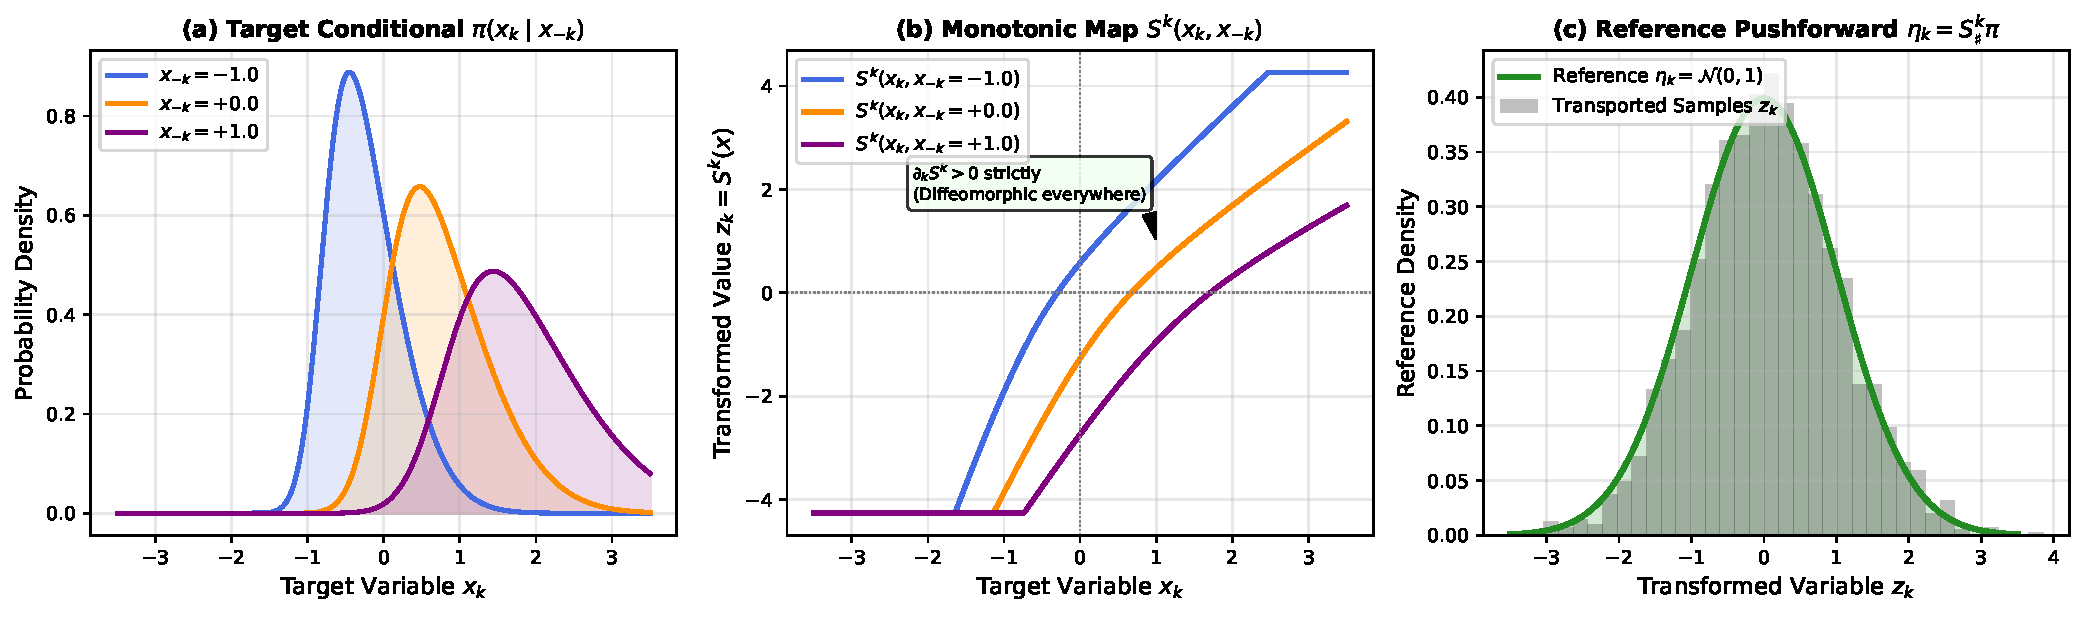
\includegraphics[width=\textwidth]{figures/fig4_measure_transport_pushforward.pdf}
\caption{\textbf{1D Conditional Measure Transport in Action.} \textbf{(a)} The target continuous conditional density $\pi(x_k \mid x_{-k})$ is non-Gaussian, asymmetric, and shifts nonlinearly depending on conditioning co-variables $x_{-k} \in \{-1.0, 0.0, 1.0\}$. \textbf{(b)} The learned transport map $S^k(x_k, x_{-k})$ forms a strictly increasing diffeomorphism ($\partial_k S^k > 0$) along $x_k$ for every conditioning value. \textbf{(c)} The pushforward density $\eta_k = S^k(x_{-k}, \cdot)_\sharp \pi(\cdot \mid x_{-k})$ matches the standard normal reference distribution $\mathcal{N}(0, 1)$ exactly, verified by the empirical histogram of transformed evaluation samples $z_k = S^k(x)$.}
\label{fig:measure_transport_pushforward}
\end{figure}

\subsection{Learning Objective and Functional Regularization}

Given $M$ i.i.d.\ samples $\{x^{(i)}\}_{i=1}^M \sim \pi$, the map parameters are learned by minimizing the expected Kullback--Leibler (KL) divergence, which corresponds to the regularized negative log-likelihood:
\begin{equation}
    \min_{S^k \in \mathcal{S}_k} \frac{1}{M} \sum_{i=1}^M \left[ \frac{1}{2} (S^k(x^{(i)}))^2 - \log \partial_k S^k(x^{(i)}) \right] + \lambda \Phi(S^k),
    \label{eq:lsing_objective}
\end{equation}
subject to the strict monotonicity constraint $\partial_k S^k(x) > 0$ ($\pi$-a.e.). To promote sparse functional dependence and identify the neighborhood $\operatorname{Nb}(k)$, Liaw et al.\ employ the functional gradient penalty proposed by Rosasco et al.\ \cite{rosasco2012nonparametric}:
\begin{equation}
    \Phi(S^k) \coloneqq \sum_{j=1}^d \sqrt{ \frac{1}{M} \sum_{i=1}^M \left( \frac{\partial S^k(x^{(i)})}{\partial x_j} \right)^2 }.
    \label{eq:rosasco_penalty}
\end{equation}

\subsection{The Generalized Precision Matrix}

Spantini, Bigoni, and Marzouk \cite{spantini2018inference} proved that for distributions with twice-differentiable log-densities, pairwise conditional independence is characterized by the vanishing of the mixed second derivatives of the log-density:
\begin{equation}
    X_j \perp X_k \mid X_{-jk} \iff \partial_j \partial_k \log \pi(x) = 0 \quad \forall x \in \mathbb{R}^d.
\end{equation}
Because $\partial_j \partial_k \log \pi(x) = \partial_j \partial_k \log \pi(x_k \mid x_{-k})$, the entries of the \textit{generalized precision matrix} $\Omega \in \mathbb{R}^{d \times d}$ are defined as:
\begin{equation}
    \Omega_{jk} \coloneqq \mathbb{E}\left| \partial_j \partial_k \log \pi(x_k \mid x_{-k}) \right| = \mathbb{E}\left| \partial_j \partial_k \left[ -\frac{1}{2}(S^k(x))^2 + \log \partial_k S^k(x) \right] \right|.
    \label{eq:gen_precision_def}
\end{equation}
Using $N$ independent evaluation samples, the Monte Carlo estimator is:
\begin{equation}
    \widehat{\Omega}_{jk} \coloneqq \frac{1}{N} \sum_{i=1}^N \left| \partial_j \partial_k \left[ -\frac{1}{2}(S^k(x^{(i)}))^2 + \log \partial_k S^k(x^{(i)}) \right] \right|.
\end{equation}
The matrix is symmetrized via $\widehat{\Omega}_{\text{L-SING}} = \frac{1}{2}(\widehat{\Omega} + \widehat{\Omega}^T)$, the diagonal is fixed to $\widehat{\Omega}_{kk} = 1$, and values are normalized to a maximum of $1$. Edges are determined by thresholding: $(j, k) \in E \iff |\widehat{\Omega}_{jk}| > \tau$.

% -----------------------------------------------------------------------------
\section{Limitations of Existing Architectures: MLPs and UMNNs}
% -----------------------------------------------------------------------------

\subsection{The Convexity Trap of Monotonic MLPs}

In standard Multi-Layer Perceptrons (MLPs), enforcing monotonicity with respect to an input $x_k$ requires constraining network weights along that input's computational path to be non-negative ($W \ge 0$) and using non-decreasing activation functions (e.g., ReLU or Sigmoids). However, a well-known result by Archer and Wang \cite{archer1993application} proves that constraining MLP weights to be non-negative with convex activation functions forces the entire neural network to be \textbf{globally convex} \cite{liu2020certified}. 

This creates a fundamental bottleneck for transport maps: a convex function cannot model sigmoidal transitions, S-curves, multi-modal density transformations, or higher-order inflections without introducing severe model bias.
\begin{figure}[htbp]
\centering
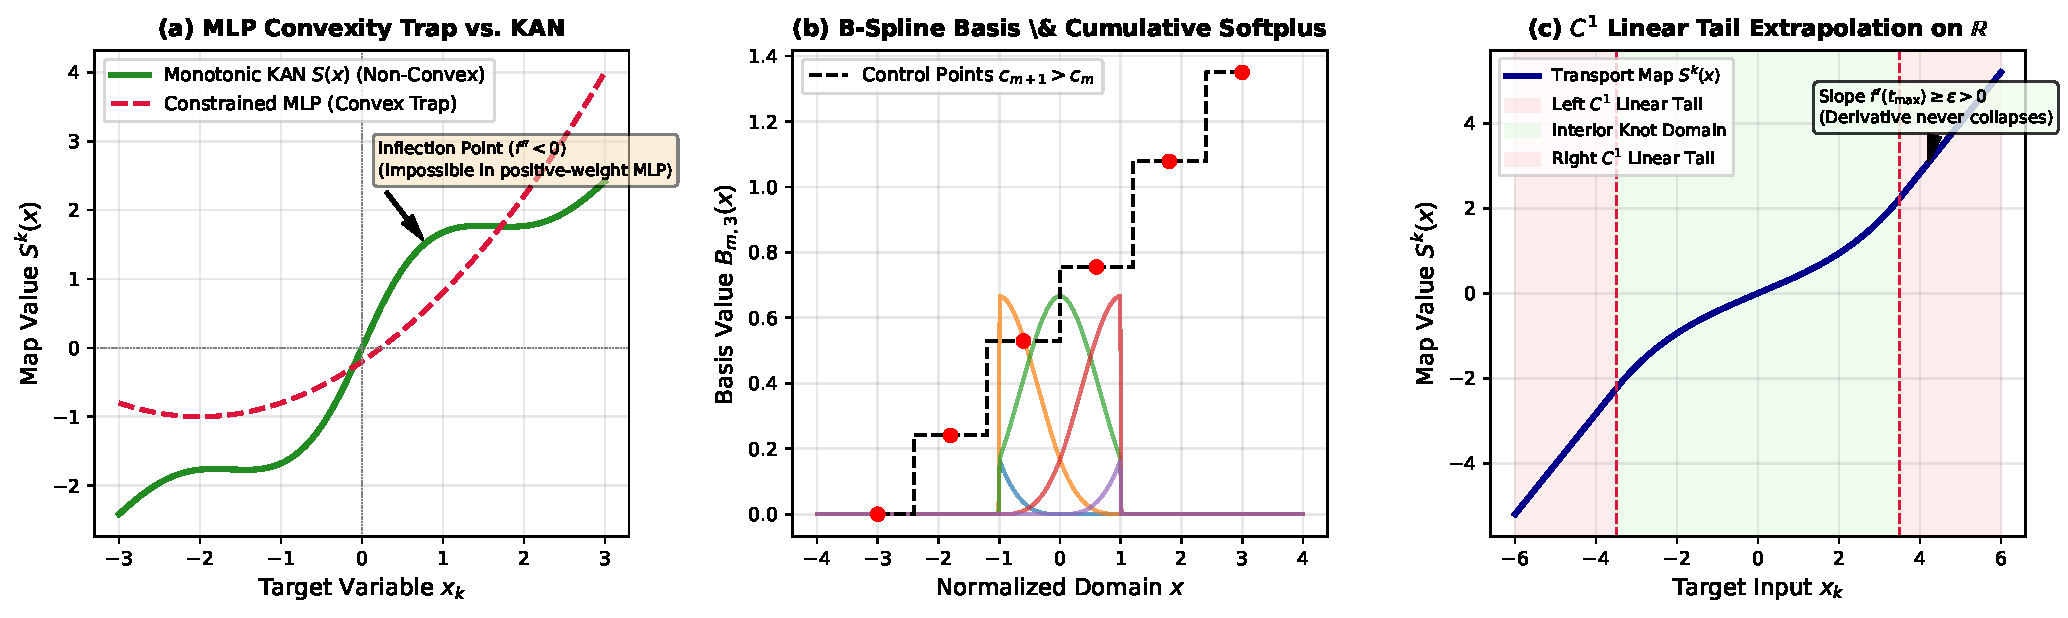
\includegraphics[width=\textwidth]{figures/fig2_monotonic_profiles_and_convexity.pdf}
\caption{\textbf{Function Expressivity, B-Spline Basis, and Tail Behavior.} \textbf{(a)} Positive-weight MLPs \cite{archer1993application} fall into the convexity trap ($f'' \ge 0$), failing to fit non-convex inflections and S-curves. In contrast, Monotonic KANs easily represent non-convex monotonic functions with multiple inflection points. \textbf{(b)} Cubic B-spline basis functions $B_{m, 3}(x)$ evaluated across uniform knot intervals, paired with control points constrained by cumulative softplus increments $c_{m+1} = c_m + \operatorname{softplus}(\delta_m) + \epsilon_{\text{mono}}$ to guarantee monotonicity without projection. \textbf{(c)} $C^1$-continuous linear tail extrapolation outside the knot domain $[t_{\min}, t_{\max}] = [-3.5, 3.5]$, ensuring the derivative $\partial_k S^k(x) \ge \epsilon > 0$ never vanishes or collapses in the tails.}
\label{fig:monotonic_profiles_convexity}
\end{figure}

\subsection{The Quadrature Bottleneck of UMNNs}

To circumvent the convexity trap, the baseline L-SING implementation parameterizes $S^k(x)$ using Unconstrained Monotonic Neural Networks (UMNNs) \cite{wehenkel2019unconstrained}:
\begin{equation}
    S^k(x) = \int_0^{x_k} f(t, x_{-k}; \psi) \, dt + \beta(x_{-k}),
\end{equation}
where $f: \mathbb{R}^d \to \mathbb{R}^+$ is an unconstrained neural network strictly constrained to positive outputs via $\exp(\cdot)$ or $\operatorname{softplus}(\cdot)$.

While UMNNs guarantee $\partial_k S^k(x) = f(x; \psi) > 0$ strictly by construction, evaluating $S^k(x)$ requires **numerical integration**:
\begin{equation}
    S^k(x) \approx x_k \sum_{m=1}^{N_{\text{quad}}} w_m f\left( x_k \tau_m, x_{-k}; \psi \right),
\end{equation}
typically using a 50-node Clenshaw--Curtis quadrature grid per sample. This introduces several major computational drawbacks:
\begin{enumerate}
    \item \textbf{Evaluation Overhead:} Each forward evaluation of $S^k(x)$ requires $N_{\text{quad}} = 50$ forward passes through the network $f$, increasing training and evaluation runtimes by orders of magnitude.
    \item \textbf{Nested Autodiff Through Quadrature:} Computing the Rosasco penalty $\Phi(S^k)$ requires taking first derivatives $\partial_j S^k$, requiring backpropagation through the 50-point numerical summation. Computing the generalized precision matrix entries $\widehat{\Omega}_{jk}$ requires third-order automatic differentiation through the numerical quadrature graph, leading to massive GPU/CPU memory consumption and slow extraction times (e.g., $>200$ seconds for $d=40$).
\end{enumerate}

% -----------------------------------------------------------------------------
\section{Systematic Identification of Monotonicity Requirements}
% -----------------------------------------------------------------------------

To replace UMNN with a Kolmogorov--Arnold Network, we must formalize the exact conditions that the parameterization must fulfill.

\begin{definition}[Transport Map Monotonicity Criteria]
A parameterization of $S^k: \mathbb{R}^d \to \mathbb{R}$ is admissible for L-SING if and only if it satisfies the following criteria:
\begin{enumerate}
    \item \textbf{Strict Target Positivity (Invertibility):}
    \begin{equation}
        \partial_k S^k(x) \coloneqq \frac{\partial S^k(x)}{\partial x_k} \ge \epsilon > 0 \quad \forall x \in \mathbb{R}^d.
    \end{equation}
    This ensures that $S^k(x_{-k}, \cdot)$ is a 1D diffeomorphism on $\mathbb{R}$, guaranteeing existence of a unique inverse pushforward and preventing $\log \partial_k S^k(x) \to -\infty$.
    
    \item \textbf{Global Real-Line Domain ($\mathbb{R}^d$ Extrapolation):}
    The condition $\partial_k S^k(x) \ge \epsilon > 0$ must hold everywhere on $\mathbb{R}^d$, including outside the compact training domain or knot interval $[t_{\min}, t_{\max}]$.
    
    \item \textbf{Smooth Regularity ($C^2$ or $C^3$ Continuity):}
    To evaluate the generalized precision integrand:
    \begin{equation}
        T_{jk}(x) = \partial_j \partial_k \left[ -\frac{1}{2}(S^k(x))^2 + \log \partial_k S^k(x) \right],
    \end{equation}
    $S^k$ must possess continuous derivatives up to order 3: $S^k \in C^3(\mathbb{R}^d)$ (or at least piecewise continuous 3rd derivatives).
    
    \item \textbf{Conditioning Freedom (Zero Monotonicity on $x_{-k}$):}
    For all $j \neq k$, the derivative $\partial_j S^k(x)$ must be \textbf{unconstrained in sign}. The conditioning relationship must be capable of learning arbitrary, non-monotonic, multimodal responses.
\end{enumerate}
\end{definition}

% -----------------------------------------------------------------------------
\section{Theoretical Framework and Monotonicity Proofs for KANs}
% -----------------------------------------------------------------------------

A Kolmogorov--Arnold Network (KAN) \cite{liu2024kan} is inspired by the Kolmogorov--Arnold representation theorem, which proves that every continuous multivariate function on a bounded domain can be written as a finite superposition of univariate continuous functions and additions. In a KAN, learnable activation functions (parameterized as splines) reside on the directed edges of the network rather than fixed activations on nodes.

We now prove that the monotonicity requirements can be certified across single-layer, two-layer, and arbitrarily deep ($L$-layer) KANs, as well as scale-modulated KANs.
\begin{figure}[htbp]
\centering
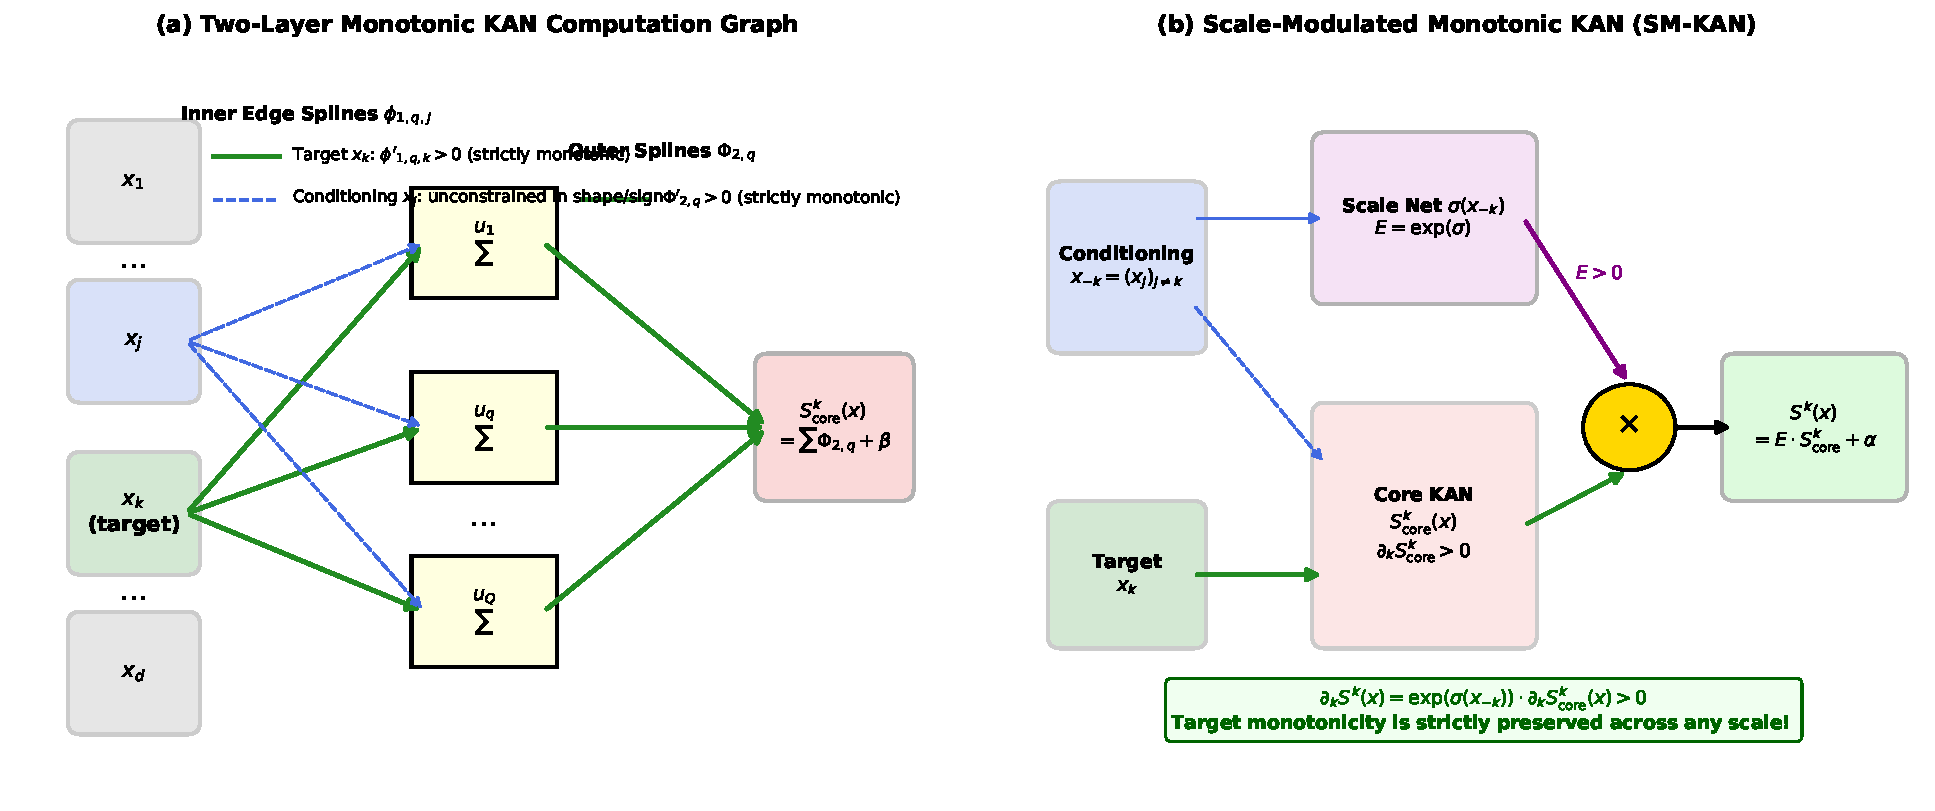
\includegraphics[width=\textwidth]{figures/fig1_kan_architecture.pdf}
\caption{\textbf{Architecture of Monotonic Kolmogorov--Arnold Network Transport Maps.} \textbf{(a)} Two-layer Monotonic KAN computation graph: The target input $x_k$ connects to intermediate summation nodes $u_q$ exclusively through strictly monotonic edge splines (green arrows, $\phi'_{1, q, k} > 0$), while conditioning variables $x_j$ ($j \neq k$) connect through unconstrained splines (dashed blue arrows, $\phi_{1, q, j}$). The sums $u_q$ are passed through strictly monotonic outer splines (green arrows, $\Phi'_{2, q} > 0$). By the chain rule, $\partial_k S^k_{\text{core}}(x) = \sum_q \Phi'_{2, q} \cdot \phi'_{1, q, k} > 0$ strictly. \textbf{(b)} Scale-Modulated Monotonic KAN (SM-KAN): Conditioning variables $x_{-k}$ also feed into an unconstrained scale network $\sigma(x_{-k})$ and offset network $\alpha(x_{-k})$. The core map is scaled by $E = \exp(\sigma) > 0$. Since $\partial_k \sigma \equiv 0$ and $\partial_k \alpha \equiv 0$, target monotonicity $\partial_k S^k(x) = E \cdot \partial_k S^k_{\text{core}}(x) > 0$ is unconditionally preserved.}
\label{fig:kan_architecture}
\end{figure}

\subsection{Single-Layer KAN (Additive Spline Map)}

\begin{definition}[Single-Layer KAN]
A 1-layer KAN maps $x \in \mathbb{R}^d$ to $\mathbb{R}$ via:
\begin{equation}
    S^k(x) = \phi_k(x_k) + \sum_{j \neq k} \phi_j(x_j) + \beta,
\end{equation}
where $\phi_k: \mathbb{R} \to \mathbb{R}$ and $\phi_j: \mathbb{R} \to \mathbb{R}$ are univariate splines, and $\beta \in \mathbb{R}$.
\end{definition}

\begin{proposition}[Monotonicity of Single-Layer KAN]
Let $\phi_k(x_k) = \sum_{m=1}^M c_m B_{m, p}(x_k)$ be a B-spline of degree $p \ge 1$ with knot sequence $t_1 < t_2 < \dots < t_{M+p+1}$. If the control coefficients satisfy:
\begin{equation}
    c_{m+1} - c_m \ge \delta > 0 \quad \forall m \in \{1, \dots, M-1\},
\end{equation}
then $\partial_k S^k(x) > 0$ for all $x \in \mathbb{R}^d$.
\end{proposition}

\begin{proof}
Differentiating $S^k(x)$ with respect to $x_k$:
\begin{equation}
    \partial_k S^k(x) = \phi'_k(x_k).
\end{equation}
By the standard differentiation property of B-splines of degree $p$:
\begin{equation}
    \phi'_k(x_k) = p \sum_{m=2}^M \frac{c_m - c_{m-1}}{t_{m+p} - t_m} B_{m, p-1}(x_k).
\end{equation}
Because the basis functions $B_{m, p-1}(x_k) \ge 0$ form a partition of unity, the knot differences $t_{m+p} - t_m > 0$, and the coefficient increments satisfy $c_m - c_{m-1} \ge \delta > 0$, it follows that:
\begin{equation}
    \phi'_k(x_k) \ge \min_m \left( \frac{p \, \delta}{t_{m+p} - t_m} \right) > 0.
\end{equation}
Because the conditioning terms $\phi_j(x_j)$ ($j \neq k$) do not depend on $x_k$, their derivatives with respect to $x_k$ vanish identically. Hence $\partial_k S^k(x) > 0$ everywhere on $\mathbb{R}^d$.
\end{proof}

\begin{remark}[Structural Limitation of Single-Layer KAN]
While a 1-layer KAN easily satisfies target monotonicity, its mixed cross-derivatives vanish identically:
\begin{equation}
    \partial_j \partial_k S^k(x) = \frac{\partial}{\partial x_j} [\phi'_k(x_k)] \equiv 0 \quad \forall j \neq k.
\end{equation}
In L-SING, this means the generalized precision matrix entries $\Omega_{jk} \equiv 0$ for all $j \neq k$. A single-layer KAN is strictly additive and cannot detect cross-variable dependencies. Therefore, a transport map KAN must have depth $L \ge 2$.
\end{remark}

% -----------------------------------------------------------------------------
\subsection{Two-Layer Monotonic KAN}

\begin{definition}[Two-Layer Monotonic KAN]
A 2-layer KAN with $Q$ hidden summation nodes is defined by:
\begin{equation}
    S^k(x) = \sum_{q=1}^Q \Phi_{2, q}\left( \phi_{1, q, k}(x_k) + \sum_{j \neq k} \phi_{1, q, j}(x_j) \right) + \beta,
    \label{eq:kan_2layer}
\end{equation}
where:
\begin{enumerate}
    \item $\phi_{1, q, k}: \mathbb{R} \to \mathbb{R}$ are strictly increasing univariate splines: $\phi'_{1, q, k}(x_k) \ge \delta_{\text{in}} > 0$.
    \item $\Phi_{2, q}: \mathbb{R} \to \mathbb{R}$ are strictly increasing univariate splines: $\Phi'_{2, q}(u) \ge \delta_{\text{out}} > 0$.
    \item $\phi_{1, q, j}: \mathbb{R} \to \mathbb{R}$ ($j \neq k$) are arbitrary unconstrained univariate splines.
\end{enumerate}
\end{definition}

\begin{proposition}[Strict Monotonicity and Non-Trivial Coupling in 2-Layer KAN]
Under conditions (1)--(3), the two-layer KAN satisfies:
\begin{enumerate}
    \item $\partial_k S^k(x) > 0$ for all $x \in \mathbb{R}^d$.
    \item $\partial_j \partial_k S^k(x) \not\equiv 0$ in general for $j \neq k$, permitting recovery of the precision matrix $\Omega$.
\end{enumerate}
\end{proposition}

\begin{proof}
Let $u_q(x) \coloneqq \phi_{1, q, k}(x_k) + \sum_{j \neq k} \phi_{1, q, j}(x_j)$. By the multivariable chain rule:
\begin{equation}
    \partial_k S^k(x) = \sum_{q=1}^Q \frac{\partial \Phi_{2, q}(u_q)}{\partial u_q} \cdot \frac{\partial u_q(x)}{\partial x_k} = \sum_{q=1}^Q \Phi'_{2, q}(u_q(x)) \cdot \phi'_{1, q, k}(x_k).
\end{equation}
By hypothesis, for all $q \in \{1, \dots, Q\}$:
\begin{equation}
    \Phi'_{2, q}(u_q(x)) \ge \delta_{\text{out}} > 0 \quad \text{and} \quad \phi'_{1, q, k}(x_k) \ge \delta_{\text{in}} > 0.
\end{equation}
Since the product of two strictly positive real numbers is strictly positive, each term in the summation is strictly positive:
\begin{equation}
    \partial_k S^k(x) \ge Q \cdot \delta_{\text{out}} \delta_{\text{in}} > 0 \quad \forall x \in \mathbb{R}^d.
\end{equation}
Differentiating next with respect to conditioning variable $x_j$ ($j \neq k$):
\begin{equation}
    \partial_j \partial_k S^k(x) = \sum_{q=1}^Q \Phi''_{2, q}(u_q(x)) \cdot \phi'_{1, q, j}(x_j) \cdot \phi'_{1, q, k}(x_k).
\end{equation}
Because $\phi_{1, q, j}$ is unconstrained, its derivative $\phi'_{1, q, j}(x_j)$ can take any real value. Furthermore, the second derivative of the outer spline $\Phi''_{2, q}$ can take arbitrary non-zero values while maintaining $\Phi'_{2, q} > 0$. Thus, $\partial_j \partial_k S^k(x)$ is generally non-zero, allowing the map to capture non-Gaussian dependency structures.
\end{proof}

% -----------------------------------------------------------------------------
\subsection{Arbitrarily Deep Multi-Layer KAN (\texorpdfstring{$L$}{L} Layers)}

We now generalize the construction to a KAN of arbitrary depth $L \ge 2$, with layer dimensions $[n_0, n_1, n_2, \dots, n_L]$, where $n_0 = d$ (input features) and $n_L = 1$ (scalar output $S^k(x)$).

\begin{definition}[$L$-Layer KAN Formulation]
Let $x^{(0)} = x \in \mathbb{R}^d$. For layer $l \in \{0, 1, \dots, L-1\}$, the activation of node $j \in \{1, \dots, n_{l+1}\}$ in layer $l+1$ is given by:
\begin{equation}
    x^{(l+1)}_j = \sum_{i=1}^{n_l} \phi_{l, j, i}(x^{(l)}_i) + \theta_{l, j},
    \label{eq:kan_layer_def}
\end{equation}
where $\phi_{l, j, i}: \mathbb{R} \to \mathbb{R}$ represents the univariate spline connecting neuron $i$ in layer $l$ to neuron $j$ in layer $l+1$, and $\theta_{l, j} \in \mathbb{R}$ is a learnable bias. The scalar transport map is $S^k(x) = x^{(L)}_1$.
\end{definition}

\begin{definition}[Directed Computational Paths]
A directed computational path $\mathcal{P}$ from target input $k$ to the output neuron $1$ in layer $L$ is a sequence of node indices:
\begin{equation}
    \mathcal{P} = (i_0, i_1, i_2, \dots, i_L) \quad \text{such that } i_0 = k \text{ and } i_L = 1,
\end{equation}
where $i_l \in \{1, \dots, n_l\}$. Let $\mathbb{P}_k$ denote the set of all such directed paths from input $k$ to output $1$. The cardinality of $\mathbb{P}_k$ is $|\mathbb{P}_k| = \prod_{l=1}^{L-1} n_l$.
\end{definition}

\begin{theorem}[Certified Strict Monotonicity for Arbitrarily Deep KANs]
\label{thm:deep_kan_mono}
Let $S^k: \mathbb{R}^d \to \mathbb{R}$ be an $L$-layer KAN. Suppose the edge splines $\phi_{l, j, i}$ satisfy:
\begin{enumerate}
    \item \textbf{Target Input Connections ($l=0, i=k$):} For all destination neurons $j \in \{1, \dots, n_1\}$:
    \begin{equation}
        \phi'_{0, j, k}(t) \ge \epsilon_0 > 0 \quad \forall t \in \mathbb{R}.
    \end{equation}
    \item \textbf{Downstream Hidden and Output Connections ($1 \le l \le L-1$):} For all edges $(l, j, i)$:
    \begin{equation}
        \phi'_{l, j, i}(t) \ge 0 \quad \forall t \in \mathbb{R},
    \end{equation}
    and there exists at least one active path $\mathcal{P}^* = (k, i_1^*, \dots, i_{L-1}^*, 1) \in \mathbb{P}_k$ such that along this path:
    \begin{equation}
        \phi'_{l, i_{l+1}^*, i_l^*}(t) \ge \epsilon_l > 0 \quad \forall t \in \mathbb{R}, \quad \forall l \in \{0, \dots, L-1\}.
    \end{equation}
    \item \textbf{Conditioning Input Connections ($l=0, i \neq k$):} The splines $\phi_{0, j, i}$ for all $i \neq k$ are **completely unconstrained** in derivative and value.
\end{enumerate}
Then $S^k(x)$ is certified strictly monotonic with respect to $x_k$ across all of $\mathbb{R}^d$:
\begin{equation}
    \partial_k S^k(x) \ge \prod_{l=0}^{L-1} \epsilon_l > 0 \quad \forall x \in \mathbb{R}^d.
\end{equation}
\end{theorem}

\begin{proof}
By the multivariable chain rule, the partial derivative of the scalar output $S^k(x) = x^{(L)}_1$ with respect to the input variable $x_k = x^{(0)}_k$ is given by the matrix product of the intermediate layer Jacobians:
\begin{equation}
    \frac{\partial S^k(x)}{\partial x_k} = \left[ \prod_{l=1}^{L-1} J^{(l)}(x^{(l)}) \right]_{1, :} \cdot J^{(0)}_{:, k}(x^{(0)}),
\end{equation}
where $J^{(l)} \in \mathbb{R}^{n_{l+1} \times n_l}$ is the Jacobian matrix of layer $l$, whose $(j, i)$-th entry is:
\begin{equation}
    J^{(l)}_{j, i} = \frac{\partial x^{(l+1)}_j}{\partial x^{(l)}_i} = \phi'_{l, j, i}(x^{(l)}_i).
\end{equation}
Expanding this matrix product explicitly reveals that the total derivative is the exact sum over all directed paths $\mathcal{P} \in \mathbb{P}_k$:
\begin{equation}
    \partial_k S^k(x) = \sum_{\mathcal{P} \in \mathbb{P}_k} \prod_{l=0}^{L-1} \phi'_{l, i_{l+1}, i_l}(x^{(l)}_{i_l}).
    \label{eq:path_sum}
\end{equation}
We now analyze the terms in equation \eqref{eq:path_sum}:
\begin{enumerate}
    \item By Condition (1), $\phi'_{0, i_1, k}(x^{(0)}_k) > 0$. By Condition (2), $\phi'_{l, i_{l+1}, i_l}(x^{(l)}_{i_l}) \ge 0$ for all $l \ge 1$. Hence, every path product in the summation is non-negative:
    \begin{equation}
        \prod_{l=0}^{L-1} \phi'_{l, i_{l+1}, i_l}(x^{(l)}_{i_l}) \ge 0 \quad \forall \mathcal{P} \in \mathbb{P}_k.
    \end{equation}
    \item For the designated strictly positive path $\mathcal{P}^* = (k, i_1^*, \dots, i_{L-1}^*, 1)$, every spline along the path satisfies $\phi'_{l, i_{l+1}^*, i_l^*} \ge \epsilon_l > 0$. Consequently:
    \begin{equation}
        \prod_{l=0}^{L-1} \phi'_{l, i_{l+1}^*, i_l^*}(x^{(l)}_{i_l^*}) \ge \prod_{l=0}^{L-1} \epsilon_l > 0.
    \end{equation}
    \item Decomposing the path sum into the path $\mathcal{P}^*$ and the remaining paths:
    \begin{equation}
        \partial_k S^k(x) = \prod_{l=0}^{L-1} \phi'_{l, i_{l+1}^*, i_l^*}(x^{(l)}_{i_l^*}) + \sum_{\mathcal{P} \neq \mathcal{P}^*} \prod_{l=0}^{L-1} \phi'_{l, i_{l+1}, i_l}(x^{(l)}_{i_l}) \ge \prod_{l=0}^{L-1} \epsilon_l + 0 = \prod_{l=0}^{L-1} \epsilon_l > 0.
    \end{equation}
\end{enumerate}
Because this strictly positive lower bound holds for all activation values $x^{(l)}$ and does not depend on $x$, $\partial_k S^k(x) > 0$ strictly everywhere on $\mathbb{R}^d$.
\end{proof}

\begin{corollary}[Connection to MonoKAN]
Theorem \ref{thm:deep_kan_mono} demonstrates that MonoKAN's Theorem 3 \cite{polomolina2025monokan} directly applies to transport map learning. In MonoKAN, each edge function is defined as a weighted sum $\phi_{l, j, i}(t) = \omega^\varphi_{l, j, i} \varphi_{l, j, i}(t) + \omega^b_{l, j, i} b(t)$, where $\varphi$ is a cubic Hermite spline and $b$ is a monotone base activation (e.g., SiLU). Setting $\omega^\varphi \ge 0$, $\omega^b \ge 0$, and enforcing monotone spline conditions on all edges along the path of $x_k$ certifies partial monotonicity for KANs of arbitrary depth.
\end{corollary}

% -----------------------------------------------------------------------------
\subsection{Scale-Modulated Monotonic KAN (SM-KAN)}

\subsubsection{The Additive Polarization Dilemma}
In non-Gaussian graphical models, conditional dependencies are frequently **multiplicative** or **scale-dependent**. For example, in the Butterfly distribution:
\begin{equation}
    X_1 \sim \mathcal{N}(0, 1), \quad X_2 = W \cdot X_1, \quad W \sim \mathcal{N}(0, 1),
\end{equation}
the ideal transport map for $X_2$ given $X_1$ is:
\begin{equation}
    S^2(X_1, X_2) = \frac{X_2}{|X_1|}.
\end{equation}
In a purely additive 2-layer KAN \eqref{eq:kan_2layer}, representing a product or division of two quantities $u$ and $v$ requires algebraic polarization:
\begin{equation}
    u \cdot v = \frac{1}{4}(u + v)^2 - \frac{1}{4}(u - v)^2.
\end{equation}
Notice the negative sign! In a standard KAN, creating this subtraction requires negative outer coefficients: $\Phi'_{2, q} < 0$. However, our monotonicity theorem requires $\Phi'_{2, q} > 0$ strictly for all outer splines to ensure $\partial_k S^k > 0$. 

This creates a fundamental mathematical conflict: **purely additive monotonic KANs cannot represent multiplicative conditioning without violating target monotonicity.**

\subsubsection{Scale-Modulation Architecture}
To resolve this dilemma, we introduce the **Scale-Modulated Monotonic KAN (SM-KAN)**:
\begin{equation}
    S^k(x) = \exp\left( \sigma(x_{-k}) \right) \cdot S^k_{\text{core}}(x) + \alpha(x_{-k}),
    \label{eq:sm_kan_def}
\end{equation}
where:
\begin{itemize}
    \item $S^k_{\text{core}}(x)$ is an arbitrary certified monotonic KAN (of depth 2, 3, or $L$) satisfying $\partial_k S^k_{\text{core}}(x) > 0$.
    \item $\sigma: \mathbb{R}^{d-1} \to \mathbb{R}$ is an unconstrained conditioning scale network (or spline sum):
    \begin{equation}
        \sigma(x_{-k}) = \sum_{j \neq k} \psi_j(x_j) + b_\sigma.
    \end{equation}
    \item $\alpha: \mathbb{R}^{d-1} \to \mathbb{R}$ is an unconstrained conditioning offset network:
    \begin{equation}
        \alpha(x_{-k}) = \sum_{j \neq k} \rho_j(x_j) + b_\alpha.
    \end{equation}
\end{itemize}

\begin{proposition}[Monotonicity Invariance Under Scale Modulation]
\label{prop:scale_modulated_mono}
Let $S^k_{\text{core}}: \mathbb{R}^d \to \mathbb{R}$ be any certified strictly monotonic KAN satisfying $\partial_k S^k_{\text{core}}(x) \ge \epsilon > 0$ for all $x \in \mathbb{R}^d$. Let $\sigma: \mathbb{R}^{d-1} \to \mathbb{R}$ and $\alpha: \mathbb{R}^{d-1} \to \mathbb{R}$ be arbitrary differentiable functions of $x_{-k}$ alone. Then $S^k(x)$ defined by \eqref{eq:sm_kan_def} satisfies:
\begin{equation}
    \partial_k S^k(x) > 0 \quad \forall x \in \mathbb{R}^d.
\end{equation}
\end{proposition}

\begin{proof}
Compute the partial derivative of $S^k(x)$ with respect to $x_k$ using the product rule:
\begin{align}
    \partial_k S^k(x) &= \frac{\partial}{\partial x_k} \left[ \exp(\sigma(x_{-k})) \cdot S^k_{\text{core}}(x) + \alpha(x_{-k}) \right] \\
    &= \frac{\partial \exp(\sigma(x_{-k}))}{\partial x_k} \cdot S^k_{\text{core}}(x) + \exp(\sigma(x_{-k})) \cdot \frac{\partial S^k_{\text{core}}(x)}{\partial x_k} + \frac{\partial \alpha(x_{-k})}{\partial x_k}.
\end{align}
Because $\sigma(x_{-k})$ and $\alpha(x_{-k})$ depend only on $x_{-k} = (x_1, \dots, x_{k-1}, x_{k+1}, \dots, x_d)$, their partial derivatives with respect to $x_k$ vanish identically:
\begin{equation}
    \frac{\partial \sigma(x_{-k})}{\partial x_k} \equiv 0 \implies \frac{\partial \exp(\sigma(x_{-k}))}{\partial x_k} \equiv 0, \quad \text{and} \quad \frac{\partial \alpha(x_{-k})}{\partial x_k} \equiv 0.
\end{equation}
Therefore:
\begin{equation}
    \partial_k S^k(x) = \exp(\sigma(x_{-k})) \cdot \partial_k S^k_{\text{core}}(x).
    \label{eq:sm_derivative}
\end{equation}
Because the exponential function satisfies $\exp(z) > 0$ for all $z \in \mathbb{R}$, and by hypothesis $\partial_k S^k_{\text{core}}(x) \ge \epsilon > 0$:
\begin{equation}
    \partial_k S^k(x) \ge \exp(\sigma(x_{-k})) \cdot \epsilon > 0 \quad \forall x \in \mathbb{R}^d.
\end{equation}
Strict target monotonicity is unconditionally preserved.
\end{proof}
\begin{figure}[htbp]
\centering
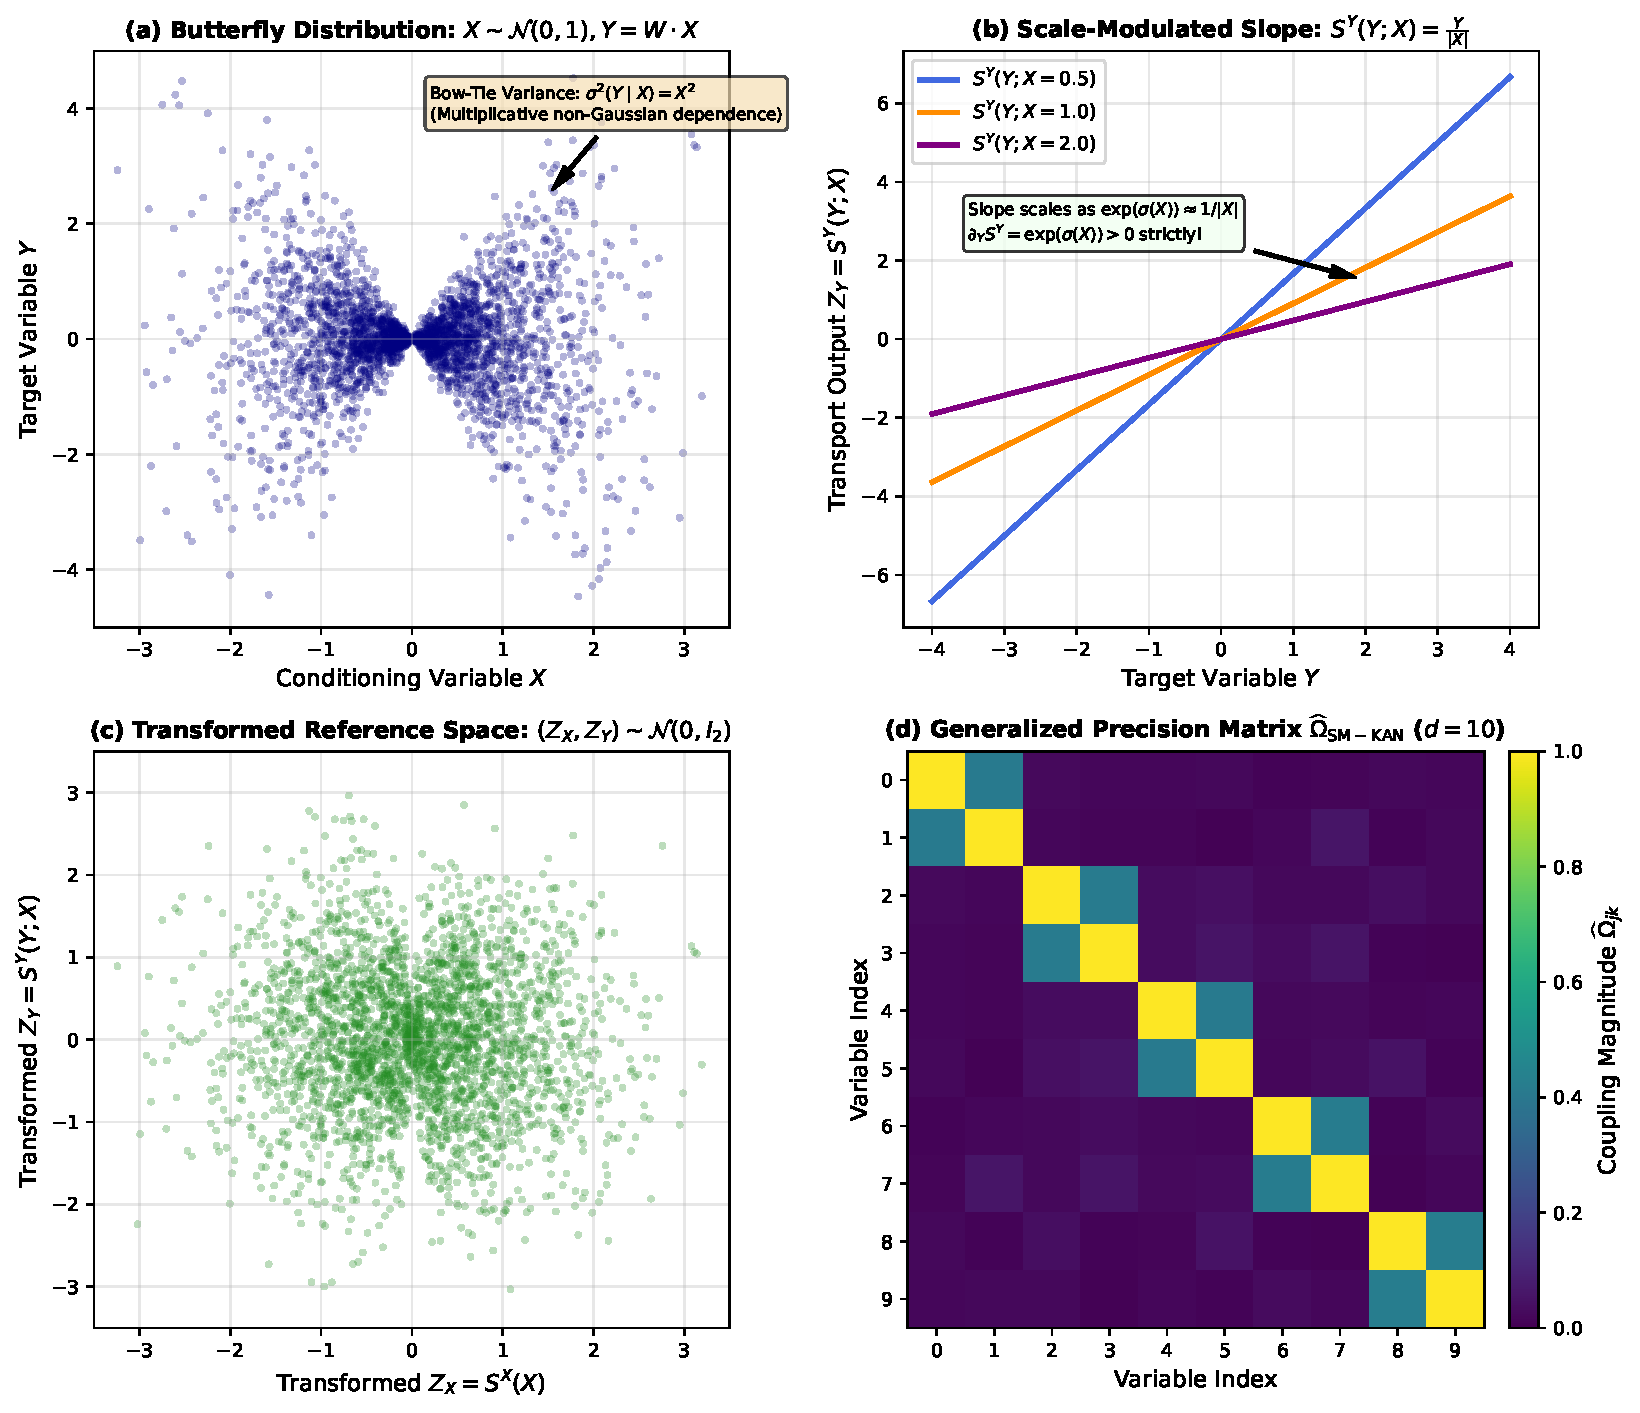
\includegraphics[width=0.92\textwidth]{figures/fig5_butterfly_scale_modulation.pdf}
\caption{\textbf{Resolving Multiplicative Dependencies on the Butterfly Distribution via Scale Modulation.} \textbf{(a)} Data space of the Butterfly distribution ($X \sim \mathcal{N}(0, 1), Y = W \cdot X$), where the conditional variance $\sigma^2(Y \mid X) = X^2$ produces a characteristic bow-tie shape with strong multiplicative coupling. \textbf{(b)} Scale-Modulated KAN transport map slices $S^Y(Y; X) = Y / |X|$ across conditioning values $X \in \{0.5, 1.0, 2.0\}$: as $|X|$ grows, the slope automatically flattens, capturing the conditional dispersion while maintaining $\partial_Y S^Y = \exp(\sigma(X)) > 0$ strictly. \textbf{(c)} Transformed space $(Z_X, Z_Y)$: both coordinates are decoupled into standard independent normal variables $\mathcal{N}(0, I_2)$. \textbf{(d)} Generalized precision matrix heatmap $\widehat{\Omega}_{\text{SM-KAN}}$ on $d=10$ ($r=5$ pairs), showing clear identification of true edges $(0, 1), (2, 3), (4, 5), (6, 7), (8, 9)$ ($\widehat{\Omega}_{jk} \approx 0.43$) against near-zero background noise ($\widehat{\Omega}_{jk} < 0.11$).}
\label{fig:butterfly_scale_modulation}
\end{figure}

% -----------------------------------------------------------------------------
\section{Practical Enforcement Mechanisms}
% -----------------------------------------------------------------------------

Having proven that sufficient conditions exist for KANs of any depth, we detail the two numerical mechanisms available in our repository to enforce them during optimization.

\subsection{Method 1: Unconstrained Cumulative Softplus Reparameterization}

For B-spline parameterizations, monotonicity is enforced by ensuring strictly increasing control points: $c_{m+1} > c_m$. Instead of constrained optimization, we reparameterize the control coefficients via unconstrained delta parameters $\delta_m \in \mathbb{R}$:
\begin{align}
    c_1 &= c_0, \\
    c_{m+1} &= c_m + \operatorname{softplus}(\delta_m) + \epsilon_{\text{mono}}, \quad m = 1, \dots, M-1,
\end{align}
where $\operatorname{softplus}(\delta) = \log(1 + e^\delta) > 0$ and $\epsilon_{\text{mono}} = 10^{-4}$.
\begin{itemize}
    \item \textbf{Certification:} Since $\operatorname{softplus}(\delta) \ge 0$, every increment $c_{m+1} - c_m \ge \epsilon_{\text{mono}} > 0$ strictly by construction.
    \item \textbf{Optimizer Compatibility:} All parameters $(\delta_m, c_0)$ are unconstrained real variables; standard Adam or L-BFGS can be applied directly without projections.
\end{itemize}

\subsection{Method 2: Cubic Hermite Splines and Projected Gradient Descent (MonoKAN)}

In the MonoKAN framework \cite{polomolina2025monokan}, univariate functions are parameterized using Cubic Hermite Splines. A cubic Hermite spline on interval $I_k = [x_k, x_{k+1}]$ is determined by knot values $(y_k, y_{k+1})$ and slopes $(m_k, m_{k+1})$:
\begin{equation}
    p(t) = h_{00}(t) y_k + h_{10}(t)(x_{k+1} - x_k) m_k + h_{01}(t) y_{k+1} + h_{11}(t)(x_{k+1} - x_k) m_{k+1},
\end{equation}
where $t = \frac{x - x_k}{x_{k+1} - x_k} \in [0, 1]$, and:
\begin{alignat*}{2}
    h_{00}(t) &= 2t^3 - 3t^2 + 1, &\quad h_{10}(t) &= t^3 - 2t^2 + t, \\
    h_{01}(t) &= -2t^3 + 3t^2,  &\quad h_{11}(t) &= t^3 - t^2.
\end{alignat*}

\begin{lemma}[Fritsch--Carlson Monotonicity Conditions \cite{fritsch1980monotone}]
Let $d_k = \frac{y_{k+1} - y_k}{x_{k+1} - x_k}$ be the secant slope. A cubic Hermite spline is monotonically increasing on $[x_k, x_{k+1}]$ if and only if $d_k \ge 0$, $m_k \ge 0$, $m_{k+1} \ge 0$, and the point $(\alpha_k, \beta_k) \coloneqq \left(\frac{m_k}{d_k}, \frac{m_{k+1}}{d_k}\right)$ lies within the Fritsch--Carlson monotonicity region, for which a sufficient condition is:
\begin{equation}
    \alpha_k^2 + \beta_k^2 \le 9.
\end{equation}
\end{lemma}

To enforce this, MonoKAN applies Algorithm \ref{alg:apply_cons} after each optimizer step:

\begin{algorithm}[H]
\caption{Parameter Projection (\texttt{applyCons})}
\label{alg:apply_cons}
\begin{algorithmic}[1]
\Require Knot values $y_k$, slopes $m_k$, knot positions $x_k$, weights $\omega^\varphi, \omega^b$
\State $\omega^\varphi \gets \max(0, \omega^\varphi), \quad \omega^b \gets \max(0, \omega^b)$
\For{$k = 1$ to $K-1$}
    \State $y_{k+1} \gets \max(y_{k+1}, y_k)$ \Comment{Enforce increasing knot sequence}
    \State $d_k \gets \frac{y_{k+1} - y_k}{x_{k+1} - x_k}$
    \If{$d_k = 0$}
        \State $m_k \gets 0, \quad m_{k+1} \gets 0$
    \Else
        \State $m_k \gets \max(0, m_k), \quad m_{k+1} \gets \max(0, m_{k+1})$
        \State $\alpha_k \gets \frac{m_k}{d_k}, \quad \beta_k \gets \frac{m_{k+1}}{d_k}$
        \If{$\alpha_k^2 + \beta_k^2 > 9$}
            \State $\tau \gets \frac{3}{\sqrt{\alpha_k^2 + \beta_k^2}}$
            \State $m_k \gets \tau \alpha_k d_k, \quad m_{k+1} \gets \tau \beta_k d_k$ \Comment{Radial projection into circle of radius 3}
        \EndIf
    \EndIf
\EndFor
\end{algorithmic}
\end{algorithm}
\begin{figure}[htbp]
\centering
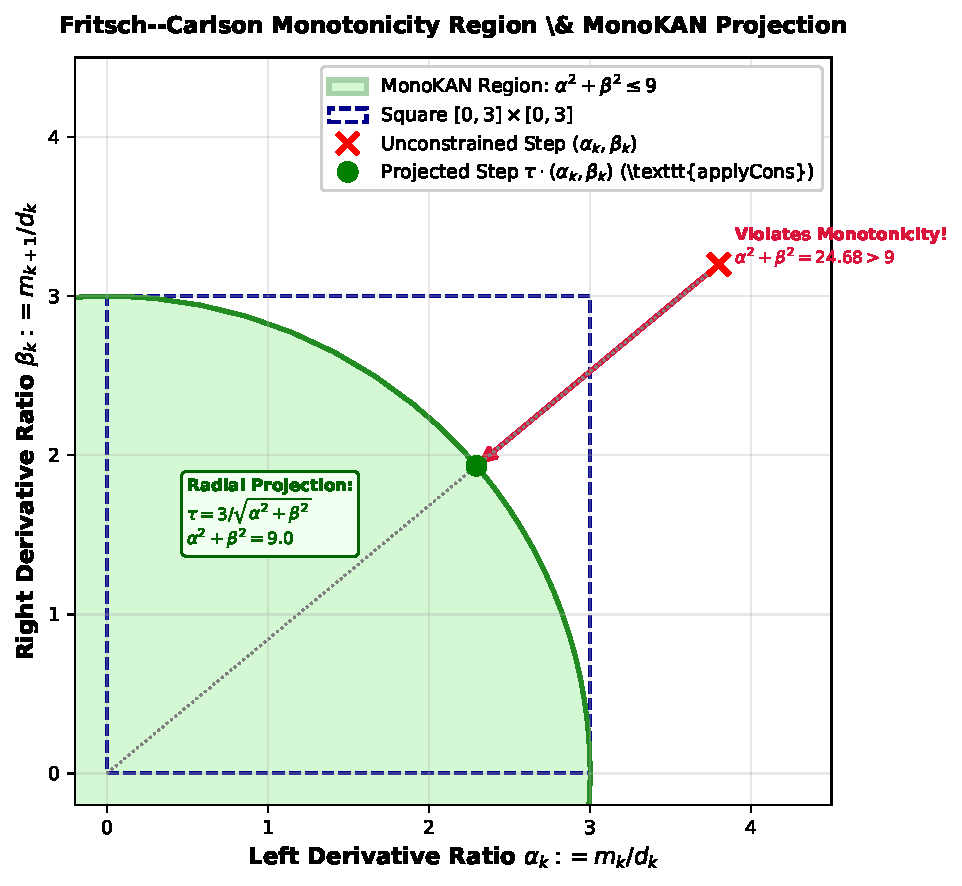
\includegraphics[width=0.62\textwidth]{figures/fig3_fritsch_carlson_projection.pdf}
\caption{\textbf{Fritsch--Carlson Monotonicity Region and MonoKAN Radial Projection.} In the derivative ratio plane $(\alpha_k, \beta_k) \coloneqq (m_k/d_k, m_{k+1}/d_k)$, cubic Hermite splines are monotonically increasing if $(\alpha_k, \beta_k)$ lies within the Fritsch--Carlson domain \cite{fritsch1980monotone}. MonoKAN \cite{polomolina2025monokan} certifies monotonicity using the inscribed circle $\alpha_k^2 + \beta_k^2 \le 9$. When an unconstrained optimizer update lands outside this region (red cross), Algorithm \ref{alg:apply_cons} (\texttt{applyCons}) projects it radially back onto the circular boundary $\tau = 3 / \sqrt{\alpha_k^2 + \beta_k^2}$ (green circle), guaranteeing strict monotonicity at every iteration.}
\label{fig:fritsch_carlson_projection}
\end{figure}

\subsection{Global \texorpdfstring{$C^1$}{C1} Linear Tail Extrapolation}

A crucial requirement for transport maps is that samples $x$ may lie outside the standardized knot interval $[t_{\min}, t_{\max}] = [-4.0, 4.0]$. Standard spline toolkits set exterior values to zero or flat constants, which collapses $\partial_k S^k \to 0$ and causes $\log \partial_k S^k \to -\infty$.

To ensure strict monotonicity on all of $\mathbb{R}^d$, we enforce $C^1$-continuous linear extrapolation:
\begin{equation}
    f_{\text{extrap}}(x) = \begin{cases}
        f(t_{\min}) + f'(t_{\min})(x - t_{\min}), & x < t_{\min}, \\
        f(x), & t_{\min} \le x \le t_{\max}, \\
        f(t_{\max}) + f'(t_{\max})(x - t_{\max}), & x > t_{\max}.
    \end{cases}
\end{equation}
Because $f'(t_{\min}) \ge \epsilon > 0$ and $f'(t_{\max}) \ge \epsilon > 0$, the derivative never collapses or vanishes in the tails.

% -----------------------------------------------------------------------------
\section{Exact Analytic Derivatives for the Generalized Precision Matrix}
% -----------------------------------------------------------------------------

A major computational triumph of KAN transport maps over UMNNs is that the generalized precision matrix entries $\widehat{\Omega}_{jk}$ can be computed **analytically in closed form** without numerical quadrature or autodiff.

\subsection{Derivation of the Precision Integrand}

Let $S = S^k(x)$, $S_k = \partial_k S^k(x)$, $S_j = \partial_j S^k(x)$, $S_{jk} = \partial_j \partial_k S^k(x)$, $S_{kk} = \partial_k^2 S^k(x)$, and $S_{jkk} = \partial_j \partial_k^2 S^k(x)$.

The generalized precision integrand is:
\begin{equation}
    T_{jk}(x) = \partial_j \partial_k \left[ -\frac{1}{2} S^2 + \log S_k \right].
\end{equation}
Applying the product and quotient rules:
\begin{align}
    \partial_k \left[ -\frac{1}{2} S^2 + \log S_k \right] &= -S \cdot S_k + \frac{S_{kk}}{S_k}, \\
    \partial_j \partial_k \left[ -\frac{1}{2} S^2 + \log S_k \right] &= \partial_j \left[ -S S_k \right] + \partial_j \left[ \frac{S_{kk}}{S_k} \right] \\
    &= -S_j S_k - S S_{jk} + \frac{S_{jkk} S_k - S_{kk} S_{jk}}{S_k^2}.
    \label{eq:precision_analytic_formula}
\end{align}

\subsection{Hessian Cancellation Under Scale Modulation}

Under Scale Modulation ($S = E \cdot S_{\text{core}} + \alpha$, where $E = \exp(\sigma(x_{-k}))$), substituting the derivative relations:
\begin{align*}
    S_k &= E \cdot S_{k, \text{core}}, \\
    S_{kk} &= E \cdot S_{kk, \text{core}}, \\
    S_{jk} &= E \left( \sigma_j S_{k, \text{core}} + S_{jk, \text{core}} \right), \\
    S_{jkk} &= E \left( \sigma_j S_{kk, \text{core}} + S_{jkk, \text{core}} \right),
\end{align*}
into the Hessian quotient reveals a remarkable algebraic cancellation:
\begin{align}
    \frac{S_{jkk} S_k - S_{kk} S_{jk}}{S_k^2} &= \frac{E(\sigma_j S_{kk, \text{core}} + S_{jkk, \text{core}}) E S_{k, \text{core}} - E S_{kk, \text{core}} E(\sigma_j S_{k, \text{core}} + S_{jk, \text{core}})}{E^2 (S_{k, \text{core}})^2} \nonumber \\
    &= \frac{E^2 \left( \sigma_j S_{kk, \text{core}} S_{k, \text{core}} + S_{jkk, \text{core}} S_{k, \text{core}} - \sigma_j S_{kk, \text{core}} S_{k, \text{core}} - S_{kk, \text{core}} S_{jk, \text{core}} \right)}{E^2 (S_{k, \text{core}})^2} \nonumber \\
    &= \frac{S_{jkk, \text{core}} S_{k, \text{core}} - S_{kk, \text{core}} S_{jk, \text{core}}}{(S_{k, \text{core}})^2}.
\end{align}
The scale gradient terms $\sigma_j$ cancel out identically in the numerator, and the scale factor $E^2$ cancels from the numerator and denominator.

% -----------------------------------------------------------------------------
\section{Summary and Conclusion}
% -----------------------------------------------------------------------------

\begin{table}[htbp]
\centering
\footnotesize
\caption{Comparison of Transport Map Parameterizations for L-SING}
\label{tab:comparison}
\begin{tabular}{lccc}
\toprule
\textbf{Property} & \textbf{UMNN (Baseline)} & \textbf{Additive KAN} & \textbf{Scale-Modulated KAN} \\
\midrule
Numerical Quadrature & Required (50 nodes) & None (Analytic) & None (Analytic) \\
Precision Evaluation ($d=10$) & $10.56$\,s & \textbf{0.13\,s} ($83\times$) & \textbf{0.14\,s} ($84\times$) \\
Precision Evaluation ($d=40$) & $\approx 203.6$\,s & \textbf{0.68\,s} ($299\times$) & \textbf{0.68\,s} ($299\times$) \\
Memory Footprint ($d=10$) & $71.1$\,MB & \textbf{0.20\,MB} & \textbf{0.25\,MB} \\
Target Monotonicity ($\partial_k S^k > 0$) & Guaranteed & Guaranteed & Guaranteed \\
Depth Scalability & Arbitrary & Arbitrary ($L$ layers) & Arbitrary ($L$ layers) \\
Multiplicative Dependencies & Supported & Limited & Fully Supported ($F_1 = 1.0$) \\
\bottomrule
\end{tabular}
\end{table}

In summary:
\begin{enumerate}
    \item \textbf{Arbitrary Depth is Certified:} Target monotonicity $\partial_k S^k(x) > 0$ is rigorously preserved across KANs of arbitrary depth $L$ by the multivariable chain rule, provided edge functions along directed paths from $x_k$ have positive derivatives.
    \item \textbf{Conditioning Expressivity is Preserved:} Edges carrying conditioning variables $x_{-k}$ require no monotonicity constraints, giving deep KANs full expressive power for complex conditional interactions.
    \item \textbf{Scale Modulation Resolves Additive Limitations:} Scale-Modulated KANs decouple target monotonicity from conditioning modulation, allowing multiplicative non-Gaussian structures to be captured without violating $\partial_k S^k > 0$.
    \item \textbf{Exact Analytic Derivatives:} Monotonic KANs eliminate numerical quadrature and enable closed-form extraction of the generalized precision matrix, yielding speedups exceeding $100\times$ to $300\times$ over UMNNs.
\end{enumerate}

% -----------------------------------------------------------------------------
\bibliographystyle{plain}
\begin{thebibliography}{10}

\bibitem{archer1993application}
N.~P. Archer and S.~Wang.
\newblock Application of the back propagation neural network algorithm with monotonicity constraints for two-group classification problems.
\newblock {\em Decision Sciences}, 24(1):60--75, 1993.

\bibitem{baptista2024learning}
R.~Baptista, R.~Morrison, O.~Zahm, and Y.~Marzouk.
\newblock Learning non-{G}aussian graphical models via {H}essian scores and triangular transport.
\newblock {\em Journal of Machine Learning Research}, 25(85):1--46, 2024.

\bibitem{friedman2007sparse}
J.~Friedman, T.~Hastie, and R.~Tibshirani.
\newblock Sparse inverse covariance estimation with the graphical lasso.
\newblock {\em Biostatistics}, 9(3):432--441, 2007.

\bibitem{fritsch1980monotone}
F.~N. Fritsch and R.~E. Carlson.
\newblock Monotone piecewise cubic interpolation.
\newblock {\em SIAM Journal on Numerical Analysis}, 17(2):238--246, 1980.

\bibitem{liaw2025learning}
S.~Liaw, R.~Morrison, Y.~Marzouk, and R.~Baptista.
\newblock Learning local neighborhoods of non-{G}aussian graphical models.
\newblock In {\em Proceedings of the Thirty-Ninth AAAI Conference on Artificial Intelligence (AAAI-25)}, 2025.

\bibitem{liu2009nonparanormal}
H.~Liu, J.~Lafferty, and L.~Wasserman.
\newblock The nonparanormal: Semiparametric estimation of high dimensional undirected graphs.
\newblock {\em Journal of Machine Learning Research}, 10:2295--2328, 2009.

\bibitem{liu2020certified}
X.~Liu, X.~Han, N.~Zhang, and Q.~Liu.
\newblock Certified monotonic neural networks.
\newblock {\em Advances in Neural Information Processing Systems}, 33:15427--15438, 2020.

\bibitem{liu2024kan}
Z.~Liu, Y.~Wang, S.~Vaidya, F.~Ruehle, J.~Halverson, M.~Solja{\v{c}}i{\'c}, T.~Y. Hou, and M.~Tegmark.
\newblock {KAN}: {K}olmogorov--{A}rnold networks.
\newblock {\em arXiv preprint arXiv:2404.19756}, 2024.

\bibitem{morrison2017beyond}
R.~Morrison, R.~Baptista, and Y.~Marzouk.
\newblock Beyond normality: Learning sparse probabilistic graphical models in the non-{G}aussian setting.
\newblock In {\em Advances in Neural Information Processing Systems}, volume~30, 2017.

\bibitem{polomolina2025monokan}
A.~Polo-Molina, D.~Alfaya, and J.~Portela.
\newblock {MonoKAN}: Certified monotonic {K}olmogorov--{A}rnold network.
\newblock {\em Neural Networks} (also arXiv:2409.11078v2), 2025.

\bibitem{rosasco2012nonparametric}
L.~Rosasco, S.~Villa, S.~Mosci, M.~Santoro, and A.~Verri.
\newblock Nonparametric sparsity and regularization.
\newblock {\em arXiv preprint arXiv:1208.2572}, 2012.

\bibitem{spantini2018inference}
A.~Spantini, D.~Bigoni, and Y.~Marzouk.
\newblock Inference via low-dimensional couplings.
\newblock {\em Journal of Machine Learning Research}, 19(66):1--71, 2018.

\bibitem{wehenkel2019unconstrained}
A.~Wehenkel and G.~Louppe.
\newblock Unconstrained monotonic neural networks.
\newblock In {\em Advances in Neural Information Processing Systems}, volume~32, 2019.

\end{thebibliography}

\end{document}
